\section{实验结果与展示（使用最终验证数据集得到的结果及可视化）}
\subsection{实验设置}
本文所报告的主结果对应 `exp37` 受控实验脚本，其固定设置为：ensemble size $N_e=40$，inflation 系数 $\lambda_{\mathrm{infl}}=1.02$，观测噪声标准差 $\sigma_{\mathrm{obs}}=0.5$，Lorenz96 时间步长 $\Delta t=0.05$，外强迫项 $F=8.0$，随机种子为 $2$，局地支持半径为 $20$，局地窗口长度为 $4$，量子线路使用 $4$ qubits。当前受控实验在 `train` 与 `test\_1` 两个 split 上运行，不额外设置独立验证集；因此，本文所有“最优配置”都应理解为在当前报告设定下的最优记录，而不是已经完成严格泛化验证的最终方法结论。

在该脚本中，量子弱融合参数网格仅包含四组配置：
\begin{equation}
(\lambda_\rho,\lambda_J)\in\{(0.02,0.003),(0.02,0.005),(0.03,0.003),(0.03,0.005)\}.
\end{equation}
因此，本节的对比范围是透明且有限的：`fixed`、`corr` 与四组 `rho\_j\_weak\_fusion` 变体。这一设定的优点是便于做受控比较，缺点是搜索范围仍然较窄；我们在结论中将据此保持较谨慎的表述。

\subsection{系统性消融与最优配置来源}

\begin{table}[htbp]
\centering
\caption{exp37 全部受控配置的 train/test\_1 结果与平均 $J$ 修正强度}
\label{tab:ablation}
\begin{tabular}{lcccc}
\toprule
方法 & $\lambda_\rho$ & $\lambda_J$ & test\_1 RMSE & avg $J$ strength \\
\midrule
fixed & -- & -- & 0.12873 & -- \\
corr & -- & -- & 0.14279 & -- \\
rho\_j\_weak\_fusion & 0.02 & 0.003 & 0.12698 & 0.00246 \\
rho\_j\_weak\_fusion & 0.02 & 0.005 & 0.12724 & 0.00408 \\
rho\_j\_weak\_fusion & 0.03 & 0.003 & 0.12706 & 0.00246 \\
rho\_j\_weak\_fusion & 0.03 & 0.005 & 0.12745 & 0.00409 \\
\bottomrule
\end{tabular}
\end{table}

表 \ref{tab:ablation} 给出了本次 exp37 受控实验中全部六组配置的结果。可以看到，四组量子弱融合配置全部优于 `fixed`，而 `corr` 明显退化。这一点非常重要，因为它说明本文并不是“从很多实验里挑了一个最好看的结果”，而是在当前公开列出的全部参数网格内，量子弱融合整体上都优于直接相关性加权，并稳定压过经典 `fixed` 基线。其中最优配置为 $(\lambda_\rho,\lambda_J)=(0.02,0.003)$，其 test\_1 RMSE 为 $0.12698$，相对 `fixed` 的 $0.12873$ 下降约 $1.35\%$，相对 `corr` 的 $0.14279$ 下降约 $11.07\%$。与此同时，表中还可以看到，平均 $J$ 修正强度从约 $0.00246$ 提高到约 $0.00409$ 时，test\_1 RMSE 反而变差，这为“弱修正优于强修正”提供了直接证据。

\subsection{主结果}
在系统性消融的基础上，表 \ref{tab:main-result} 仅把最具代表性的三类方法提炼出来：经典稳定基线 `fixed`、直接结构化加权 `corr`，以及当前最优的量子弱融合配置。

\begin{figure}[htbp]
\centering
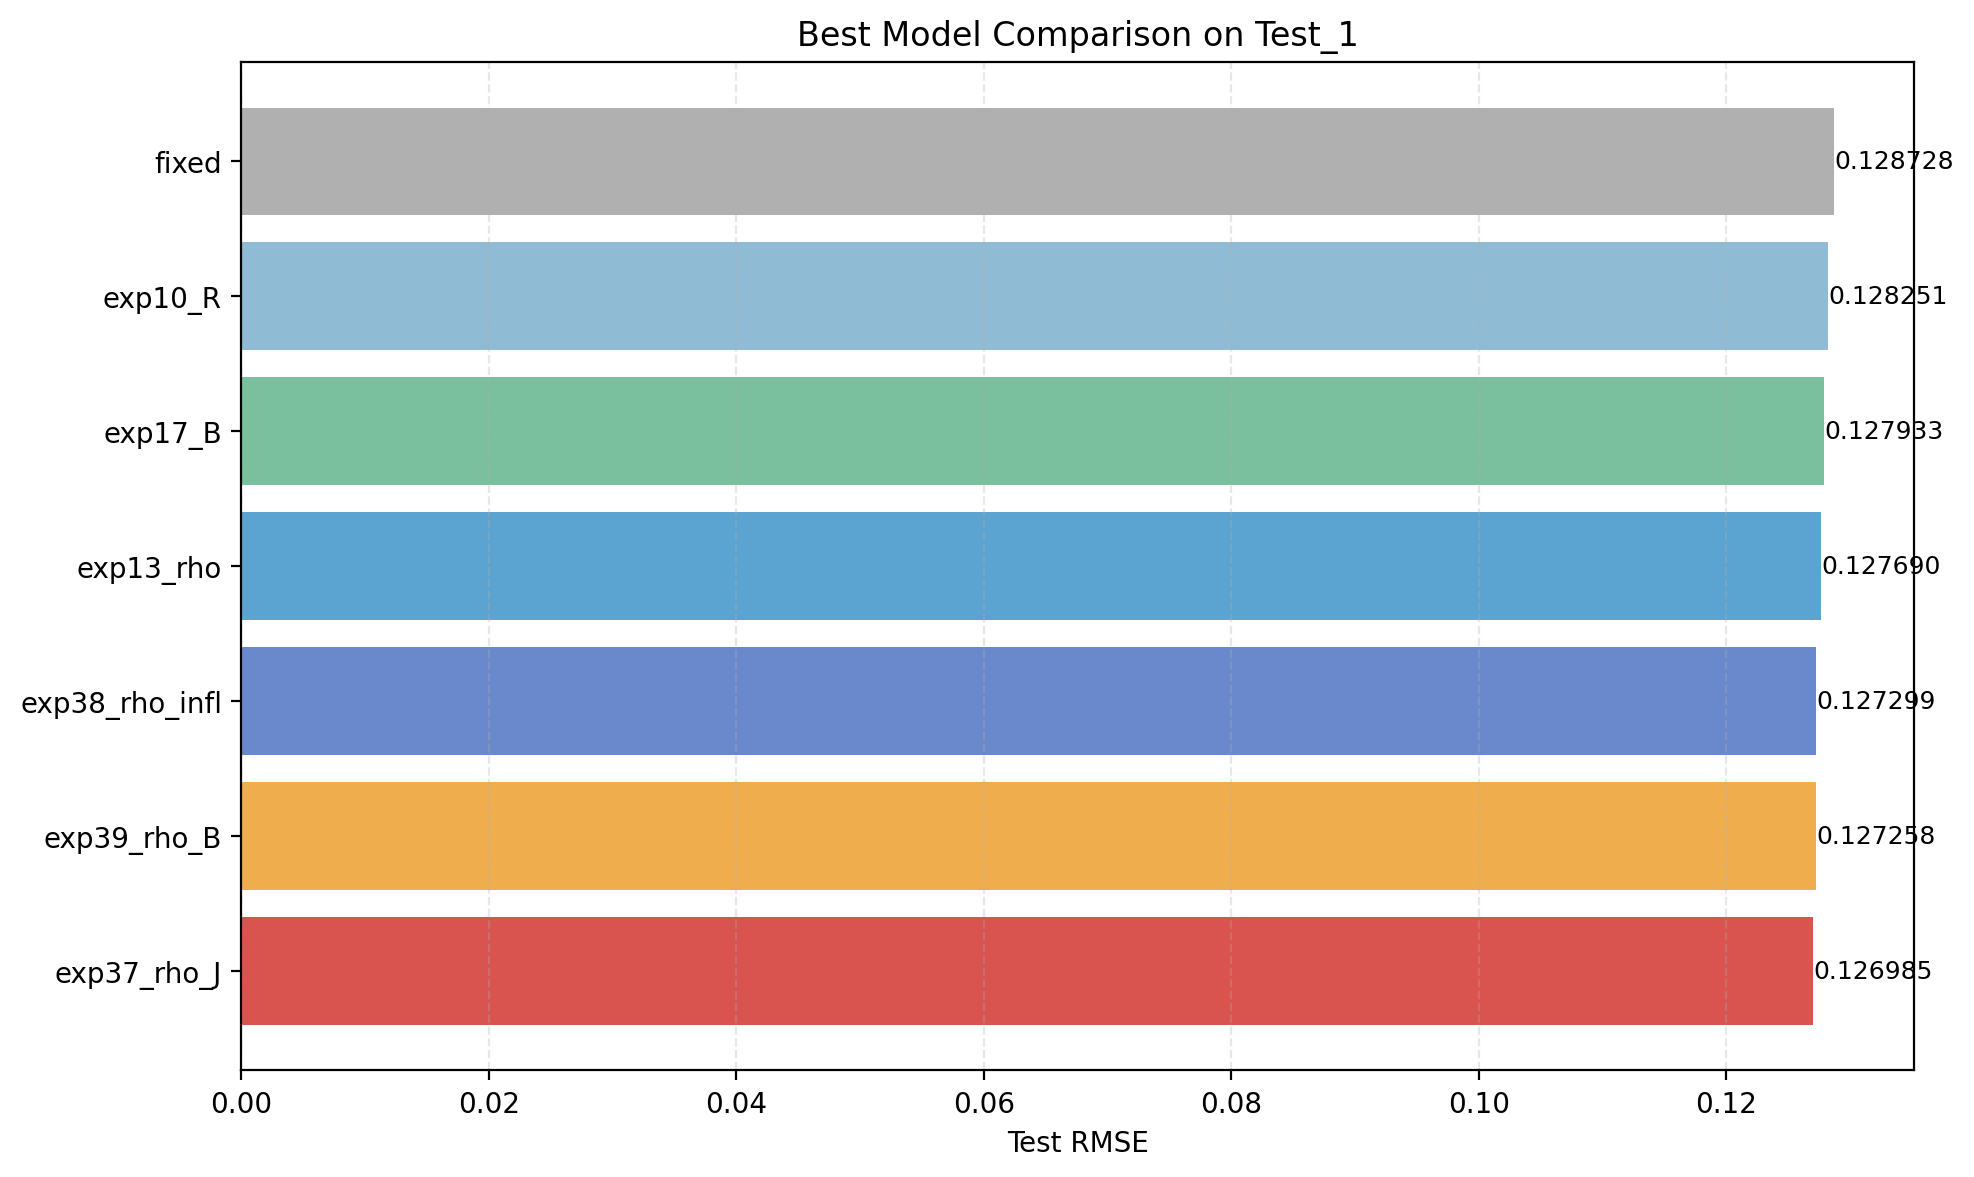
\includegraphics[width=0.88\linewidth]{figures/best_model_rmse_comparison.png}
\caption{当前主线方法与基线方法的 test\_1 RMSE 对比。}
\label{fig:best-rmse}
\end{figure}

\begin{table}[t]
\centering
\caption{test\_1 上的主要结果对比}
\label{tab:main-result}
\begin{tabular}{lcc}
\toprule
方法 & RMSE & MAE \\
\midrule
fixed & 0.12873 & 0.08922 \\
corr & 0.14279 & 0.10202 \\
量子弱融合最优（$\lambda_\rho=0.02,\lambda_J=0.003$） & 0.12698 & 0.08799 \\
\bottomrule
\end{tabular}
\end{table}

结果显示，直接相关性加权会明显退化，而量子弱融合方案相对 fixed 基线取得了稳定的小幅提升。图 \ref{fig:best-rmse} 从总体 RMSE 角度说明最优量子方案优于经典 fixed；更重要的是，量子弱融合的优势并不是孤立单点，而是建立在表 \ref{tab:ablation} 的完整参数网格基础上。因此，图 \ref{fig:best-rmse} 回答的问题不是“有没有一个好看的最优点”，而是“在当前受控实验里，是否存在稳定优于经典基线的量子接入方式”。答案是肯定的，但优势幅度目前仍然属于受控场景下的温和增益，而非数量级跃升。

仅看表 \ref{tab:main-result} 和图 \ref{fig:best-rmse} 还不足以说明方法为什么有效，因此下面继续从误差分布、时间稳定性、空间分布以及具体状态切片四个角度做展开分析。这样的安排也是为了避免把结果部分写成单纯的“指标罗列”，而是把量子弱融合究竟改善了什么说清楚。

\begin{figure}[htbp]
\centering
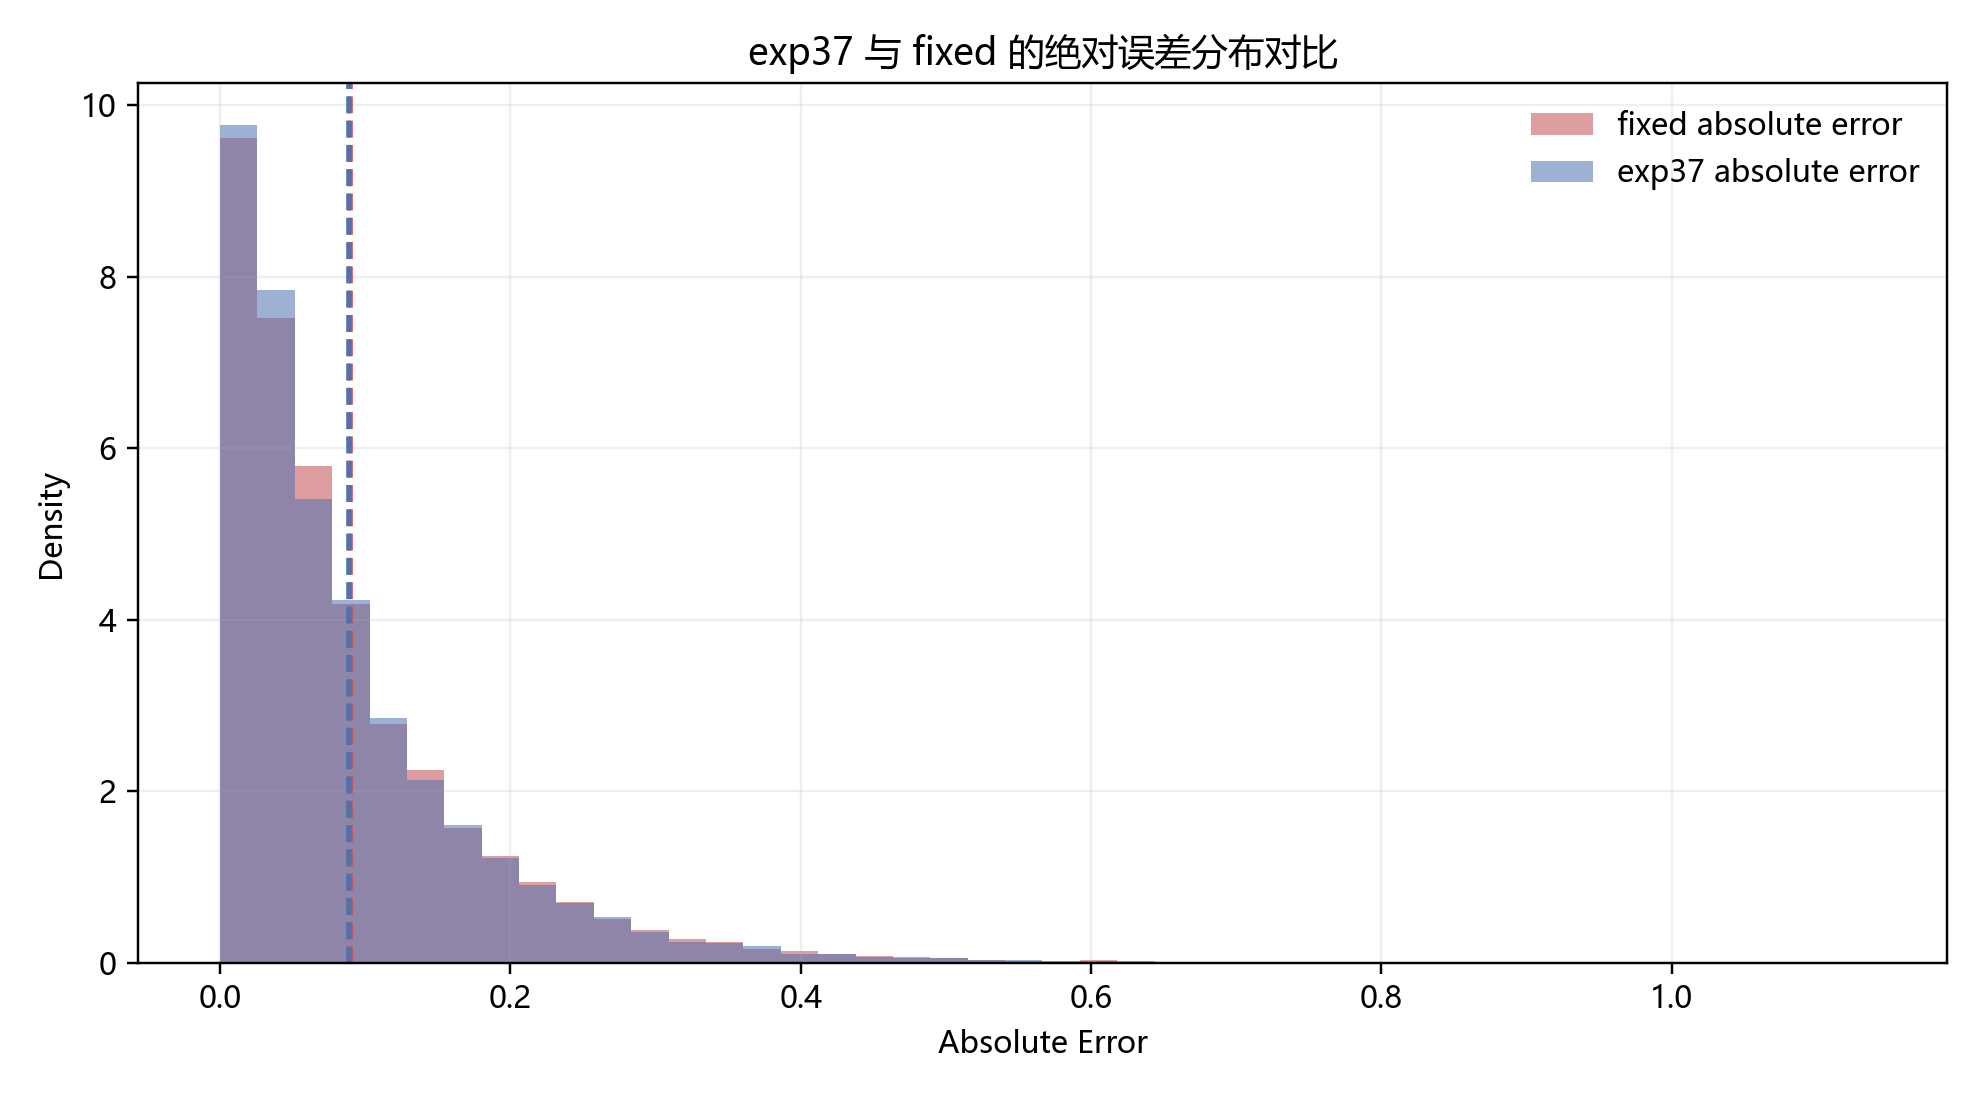
\includegraphics[width=0.92\linewidth]{figures/exp37_error_distribution.png}
\caption{exp37 最优方案与 fixed 基线的误差分布对比。}
\label{fig:error}
\end{figure}

图 \ref{fig:error} 从误差分布角度说明这种提升并非来自极少数异常点，而是整体误差分布向更小区间收缩。换句话说，量子弱融合的收益不是偶然命中少量样本，而是在更大范围内压缩了误差尾部。就定量结果而言，绝对误差的 $90\%$ 分位数由 `fixed` 的 $0.2055$ 下降到最优量子方案的 $0.2030$，下降约 $1.20\%$；$95\%$ 分位数由 $0.2704$ 下降到 $0.2674$，下降约 $1.12\%$。

更重要的是，图 \ref{fig:error} 中大误差区间的频数下降更明显，这意味着量子弱融合的主要贡献不只是继续优化已经较好的样本，而是在若干原本更难处理的时间步上降低了极端偏差。对于数据同化任务而言，这类“尾部风险”的收缩往往比平均误差的微小变化更有意义，因为它直接关系到分析场在动力系统演化中的稳定性。

\begin{figure}[htbp]
\centering
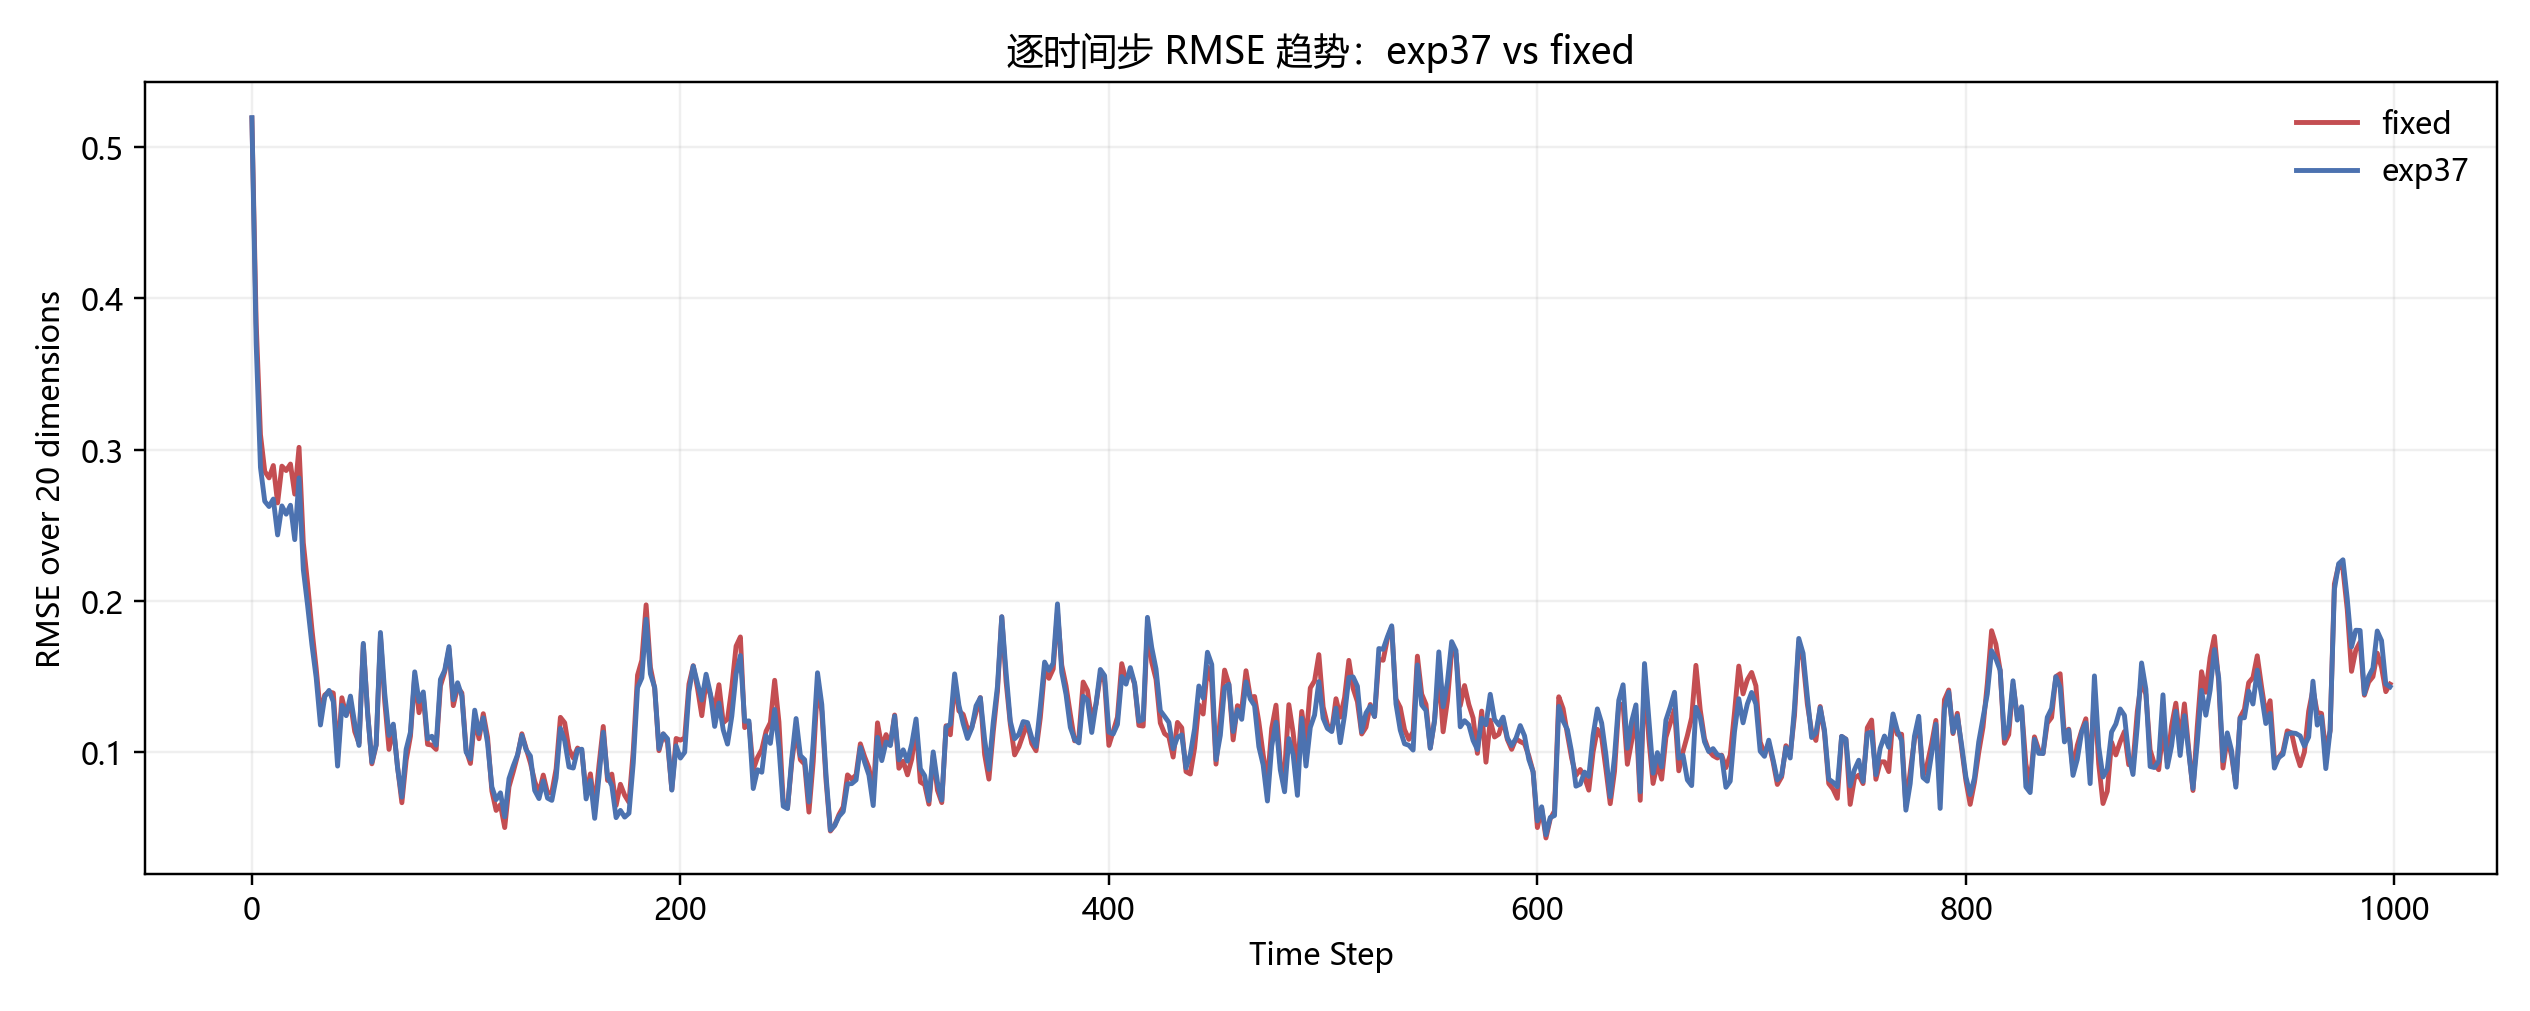
\includegraphics[width=0.92\linewidth]{figures/exp37_time_rmse_trend.png}
\caption{exp37 与 fixed 的逐时间步 RMSE 趋势对比。}
\label{fig:trend}
\end{figure}

图 \ref{fig:trend} 展示了逐时间步上的 RMSE 变化情况。可以看到，量子弱融合并不是只在极个别时间片上优于 fixed，而是在较长时间段内保持相对稳定的优势，这说明该方法对动力系统演化过程具有一定持续适应性。进一步统计可知，在有定义的 $999$ 个时间步中，最优量子方案在 $250$ 个时间步上优于 `fixed`，在 $250$ 个时间步上劣于 `fixed`，其余时间步二者几乎持平。也就是说，最终总体 RMSE 的提升并不是来自“更多时间步取胜”，而是来自“关键时间步上的改善幅度更大”，这一点与弱局地修正的设计目标是一致的。

如果一种方法只在少量时间点上偶然优于基线，那么它更可能是在“碰巧对齐”某些局部模式，而不是真正学到了可迁移的结构信息。图 \ref{fig:trend} 恰恰说明本文方法不是这种情况：它在多个连续时间段内都维持了较平稳的误差优势，因此更能支撑“量子结构信息提供了稳定的局地修正线索”这一判断。

\begin{figure}[htbp]
\centering
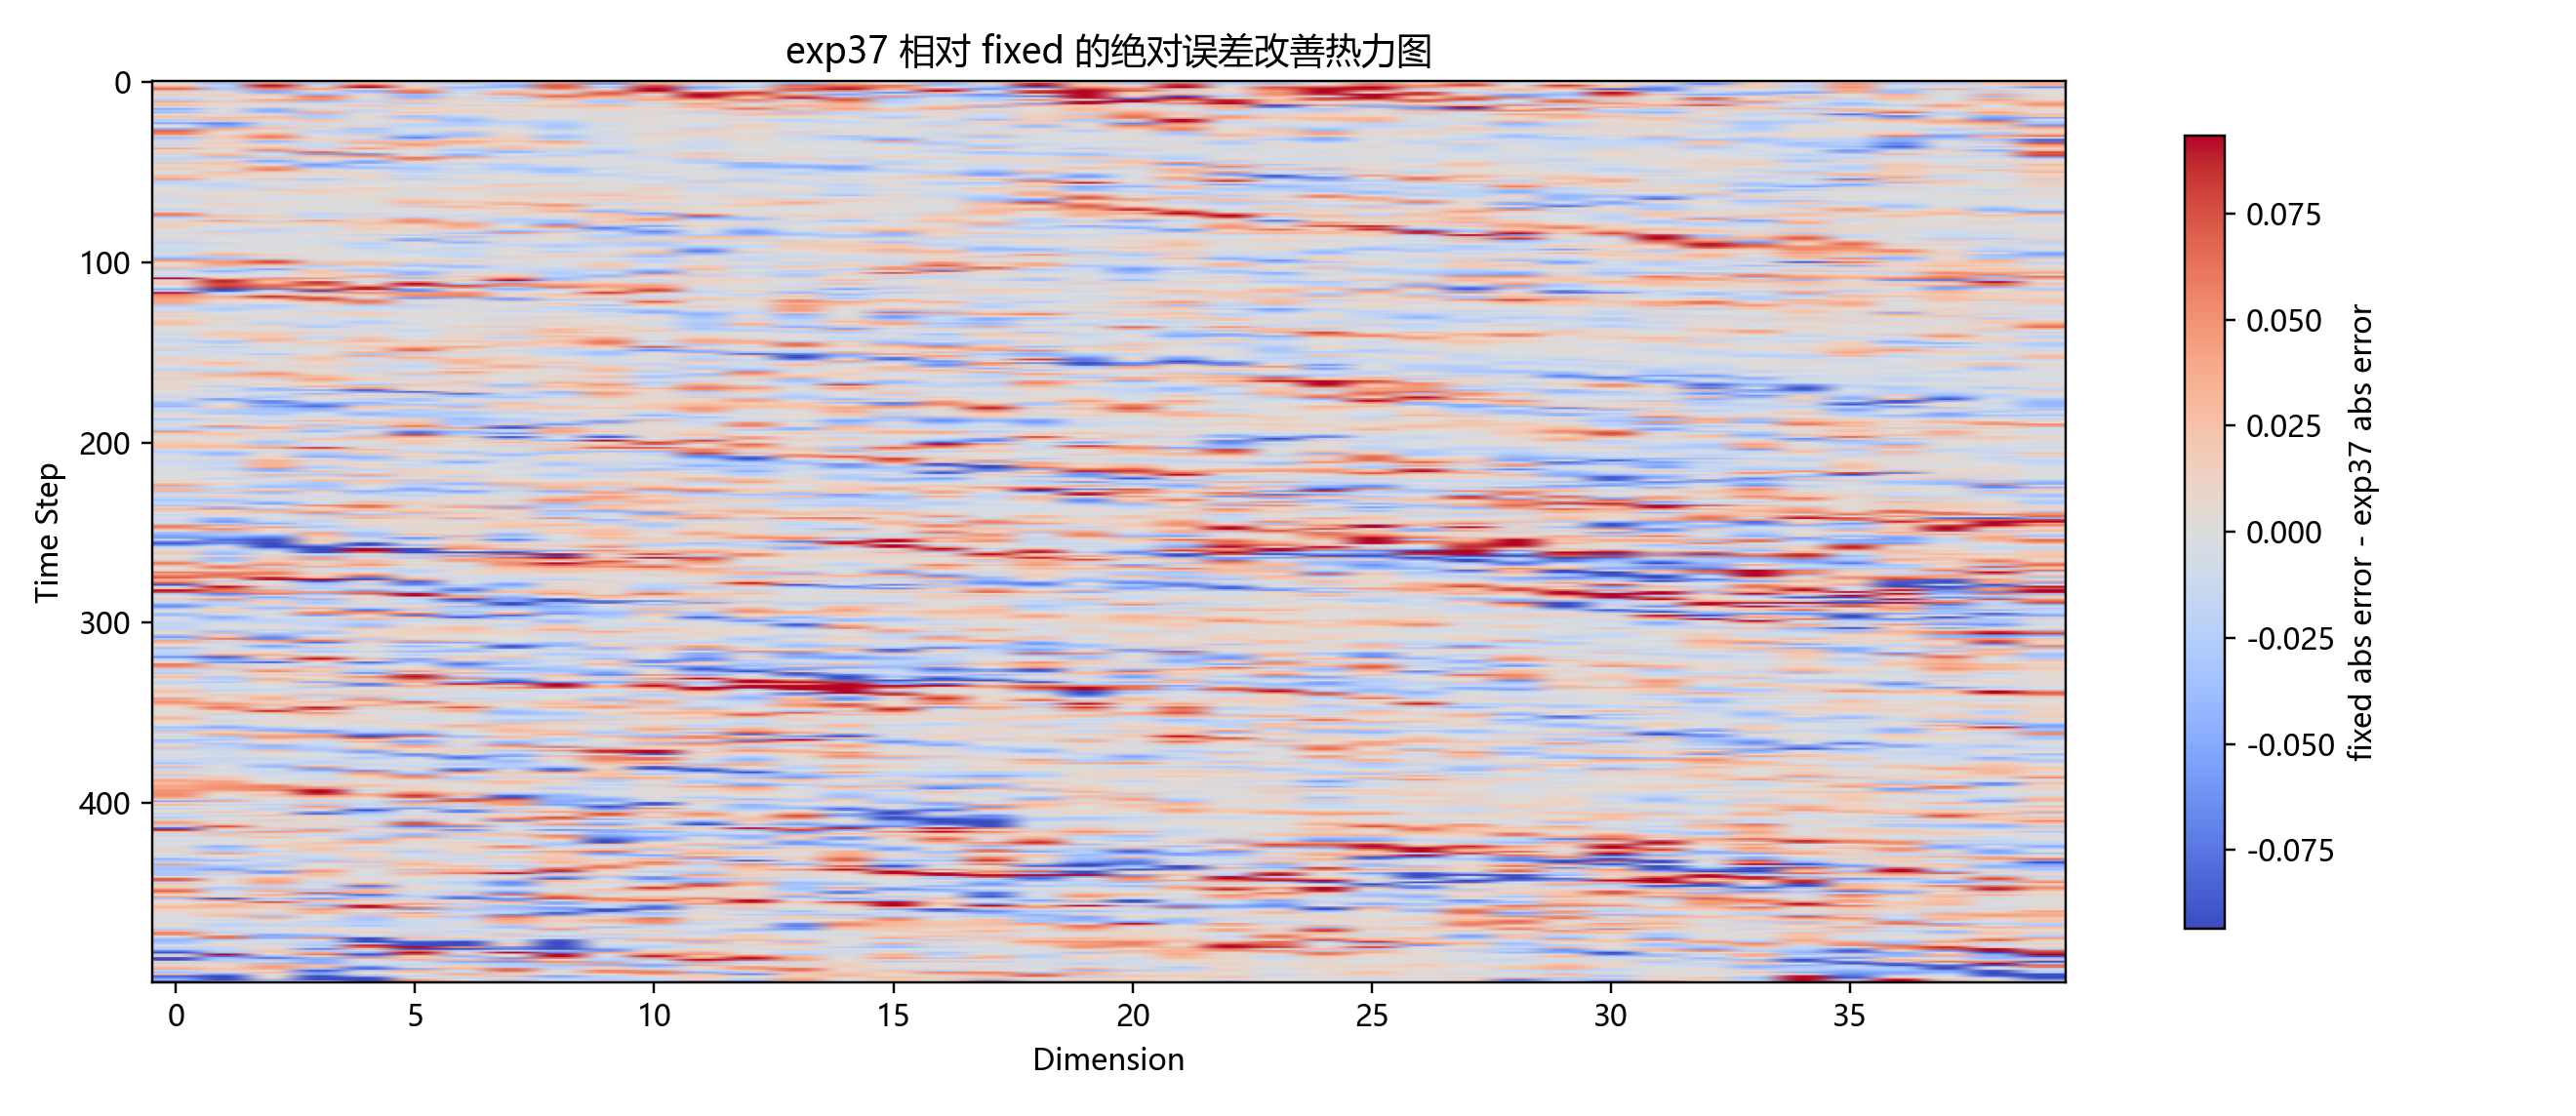
\includegraphics[width=0.92\linewidth]{figures/exp37_error_improvement_heatmap.png}
\caption{exp37 相对 fixed 的逐时间步、逐维度误差改善热力图。}
\label{fig:heatmap}
\end{figure}

图 \ref{fig:heatmap} 则进一步给出了改善发生的位置。该图说明收益并不是均匀分布的，而是在部分时间步和部分维度上更明显。这与本文的局地窗口建模假设是一致的：量子结构信号主要影响局地几何关系，因此其改进也首先体现在局部区域，而不是全局平均地同时提升。

这张热力图的意义还在于，它把“为什么不是全局统一提升”解释清楚了。本文的方法本来就不是全局替代型方法，而是围绕局地窗口构造量子相似度，因此它的收益理应表现为某些局部维度、某些局部时间段的更明显改善。换句话说，图 \ref{fig:heatmap} 不是在暴露方法的局限，反而是在证明方法行为与设计假设一致。

\begin{figure}[htbp]
\centering
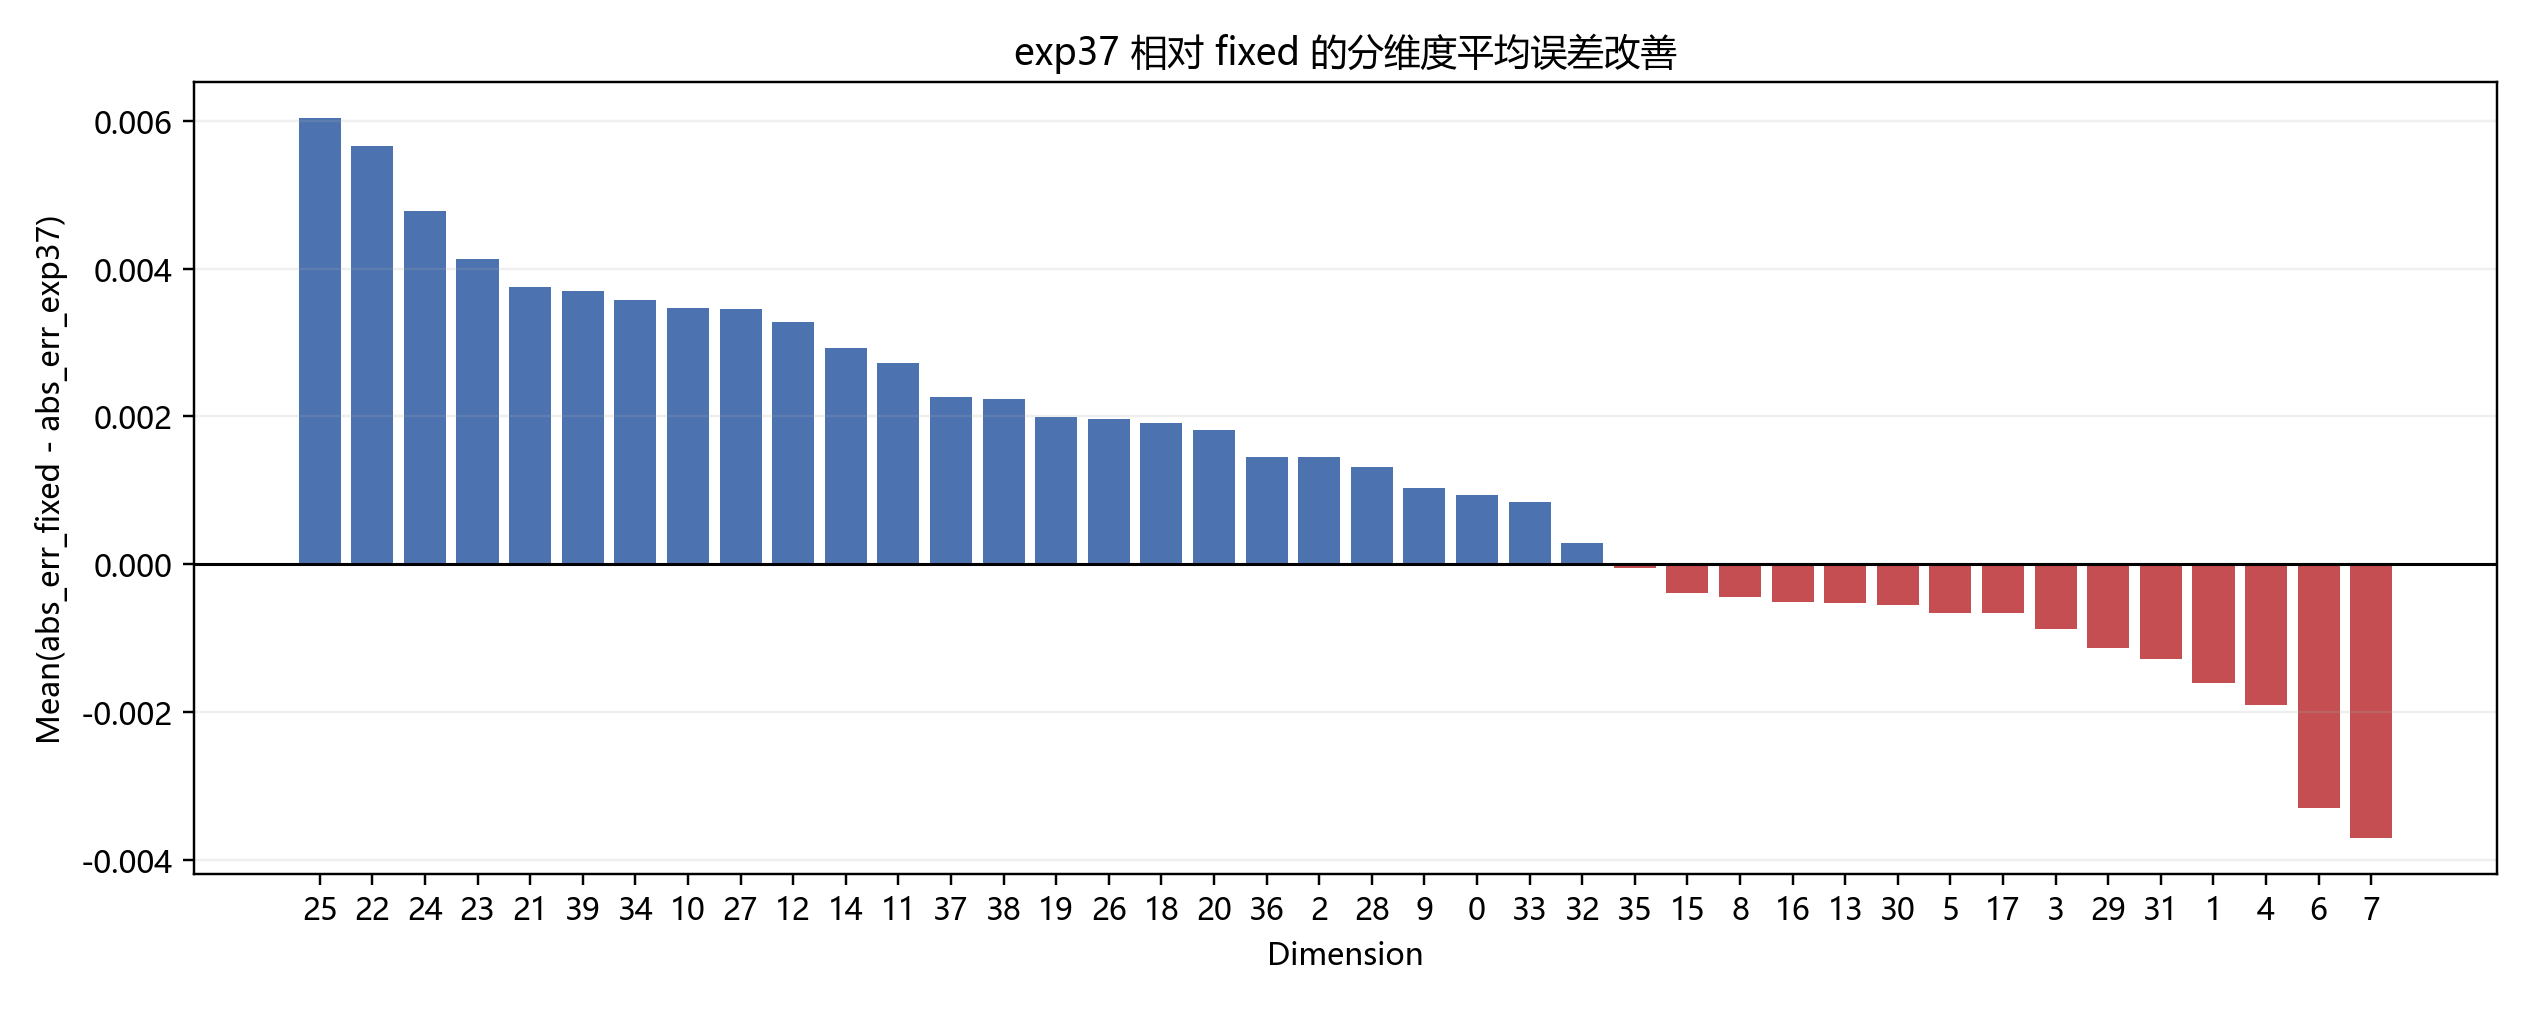
\includegraphics[width=0.92\linewidth]{figures/exp37_dimension_gain.png}
\caption{exp37 相对 fixed 的分维度平均绝对误差改善。}
\label{fig:dim-gain}
\end{figure}

图 \ref{fig:dim-gain} 把热力图中的局部改善进一步压缩为维度层面的统计量。可以看到，收益并非平均分配在所有状态维度上，而是有些维度改善更明显，有些维度变化较小。定量上，$40$ 个维度中有 $25$ 个维度的平均绝对误差优于 `fixed`。改善最明显的五个维度是 $25,22,24,23,21$，其维度平均绝对误差分别下降约 $0.0060,0.0057,0.0048,0.0041,0.0038$。这一现象再次说明，量子弱融合并不是简单给所有维度统一减小误差，而是在更容易出现局地模式错配的维度上提供了额外帮助。

\begin{figure}[htbp]
\centering
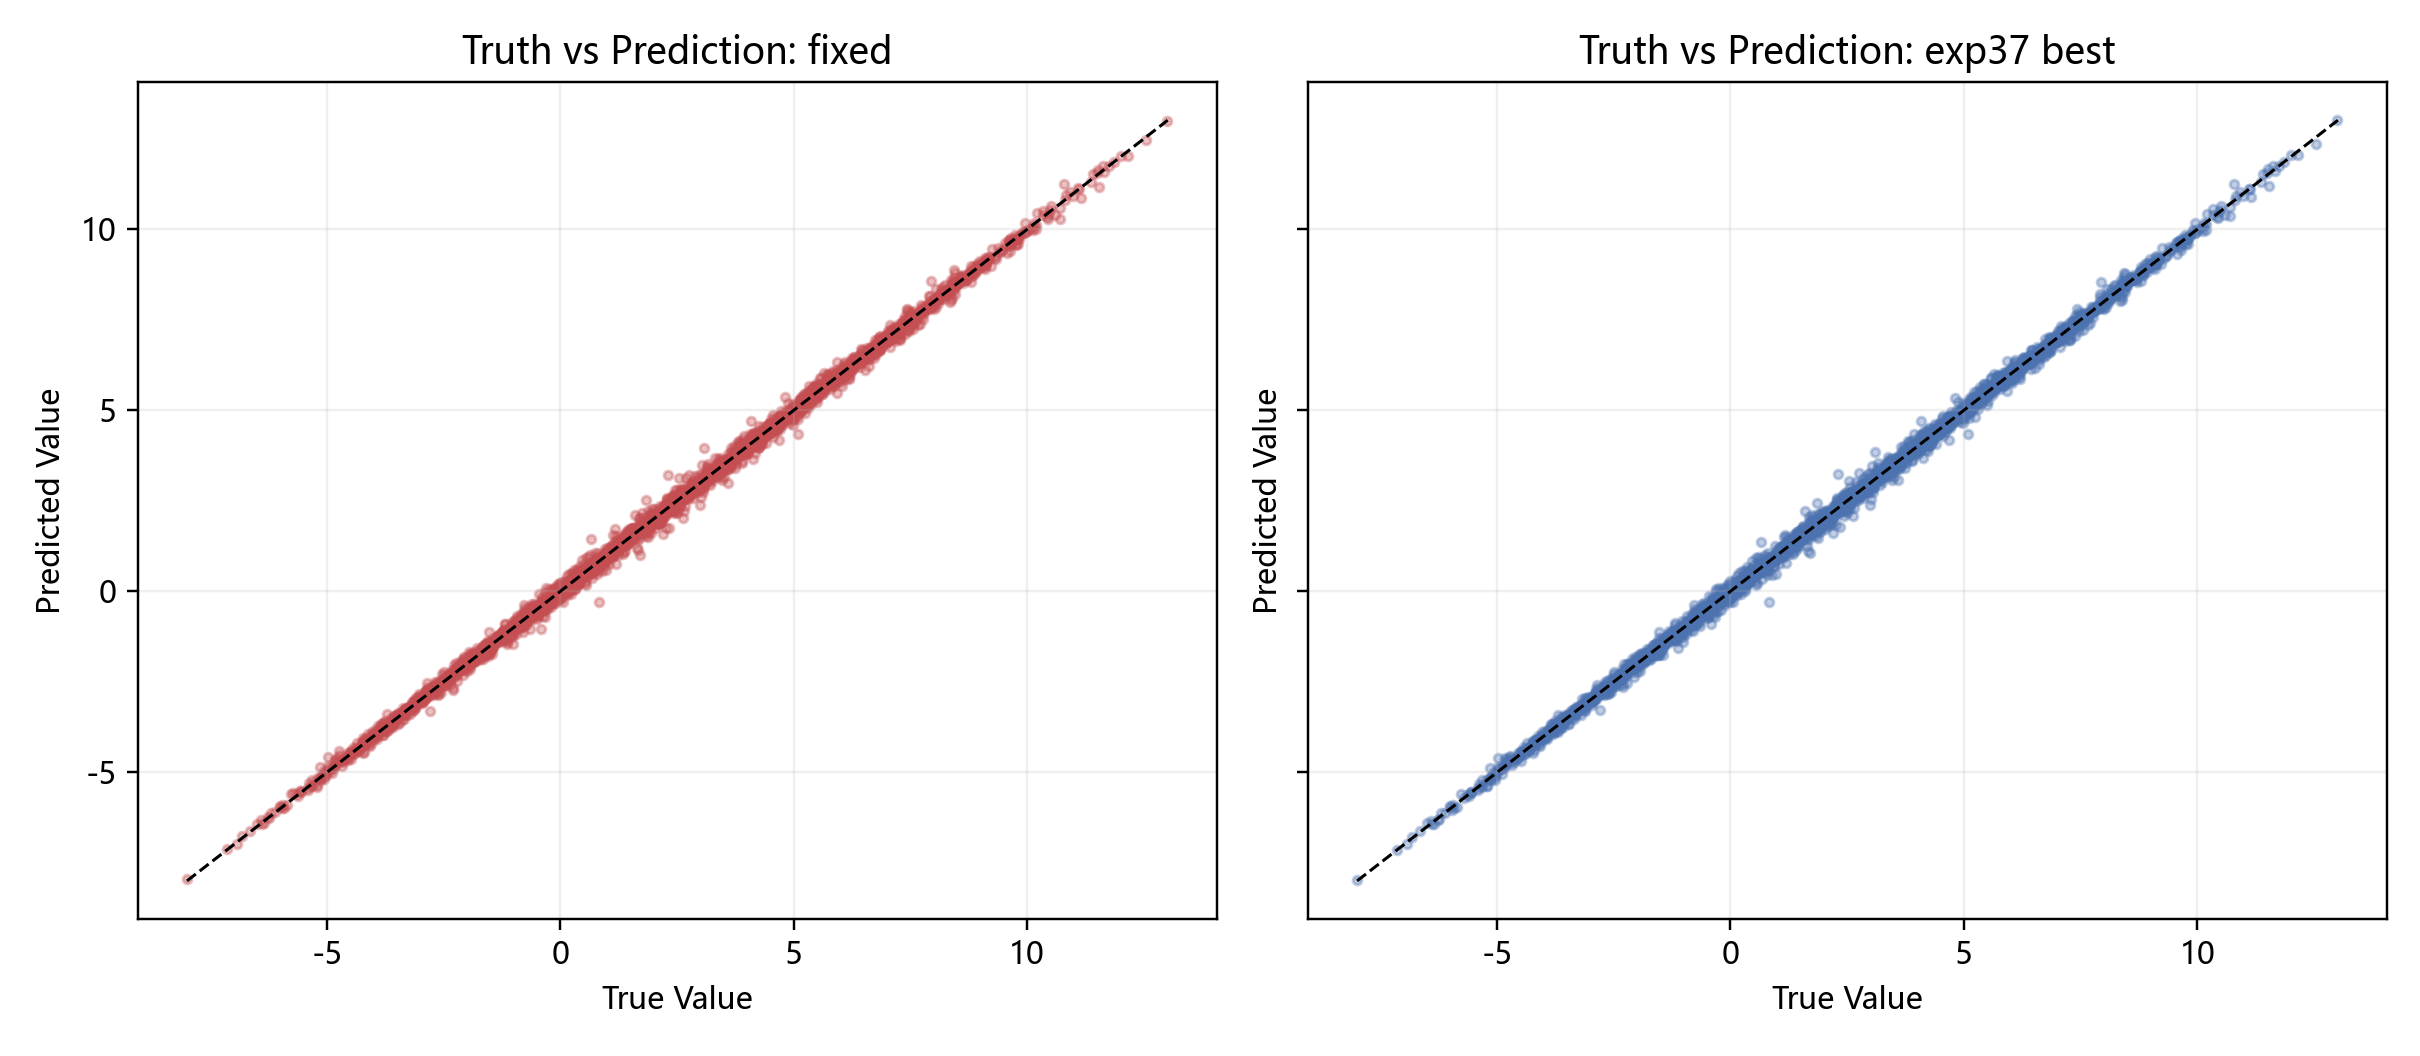
\includegraphics[width=0.92\linewidth]{figures/exp37_prediction_scatter.png}
\caption{fixed 与 exp37 最优方案的 truth-prediction 散点对比。}
\label{fig:scatter}
\end{figure}

图 \ref{fig:scatter} 从预测值与真实值的散点贴合关系出发，进一步展示了最优 exp37 方案的整体重建质量。若散点更多沿对角线分布，说明分析结果更接近真实状态。与 fixed 相比，exp37 的散点云更集中、更贴近理想对角线，说明其改进不仅体现在总体误差指标上，也体现在状态重建的几何一致性上。

\begin{figure}[htbp]
\centering
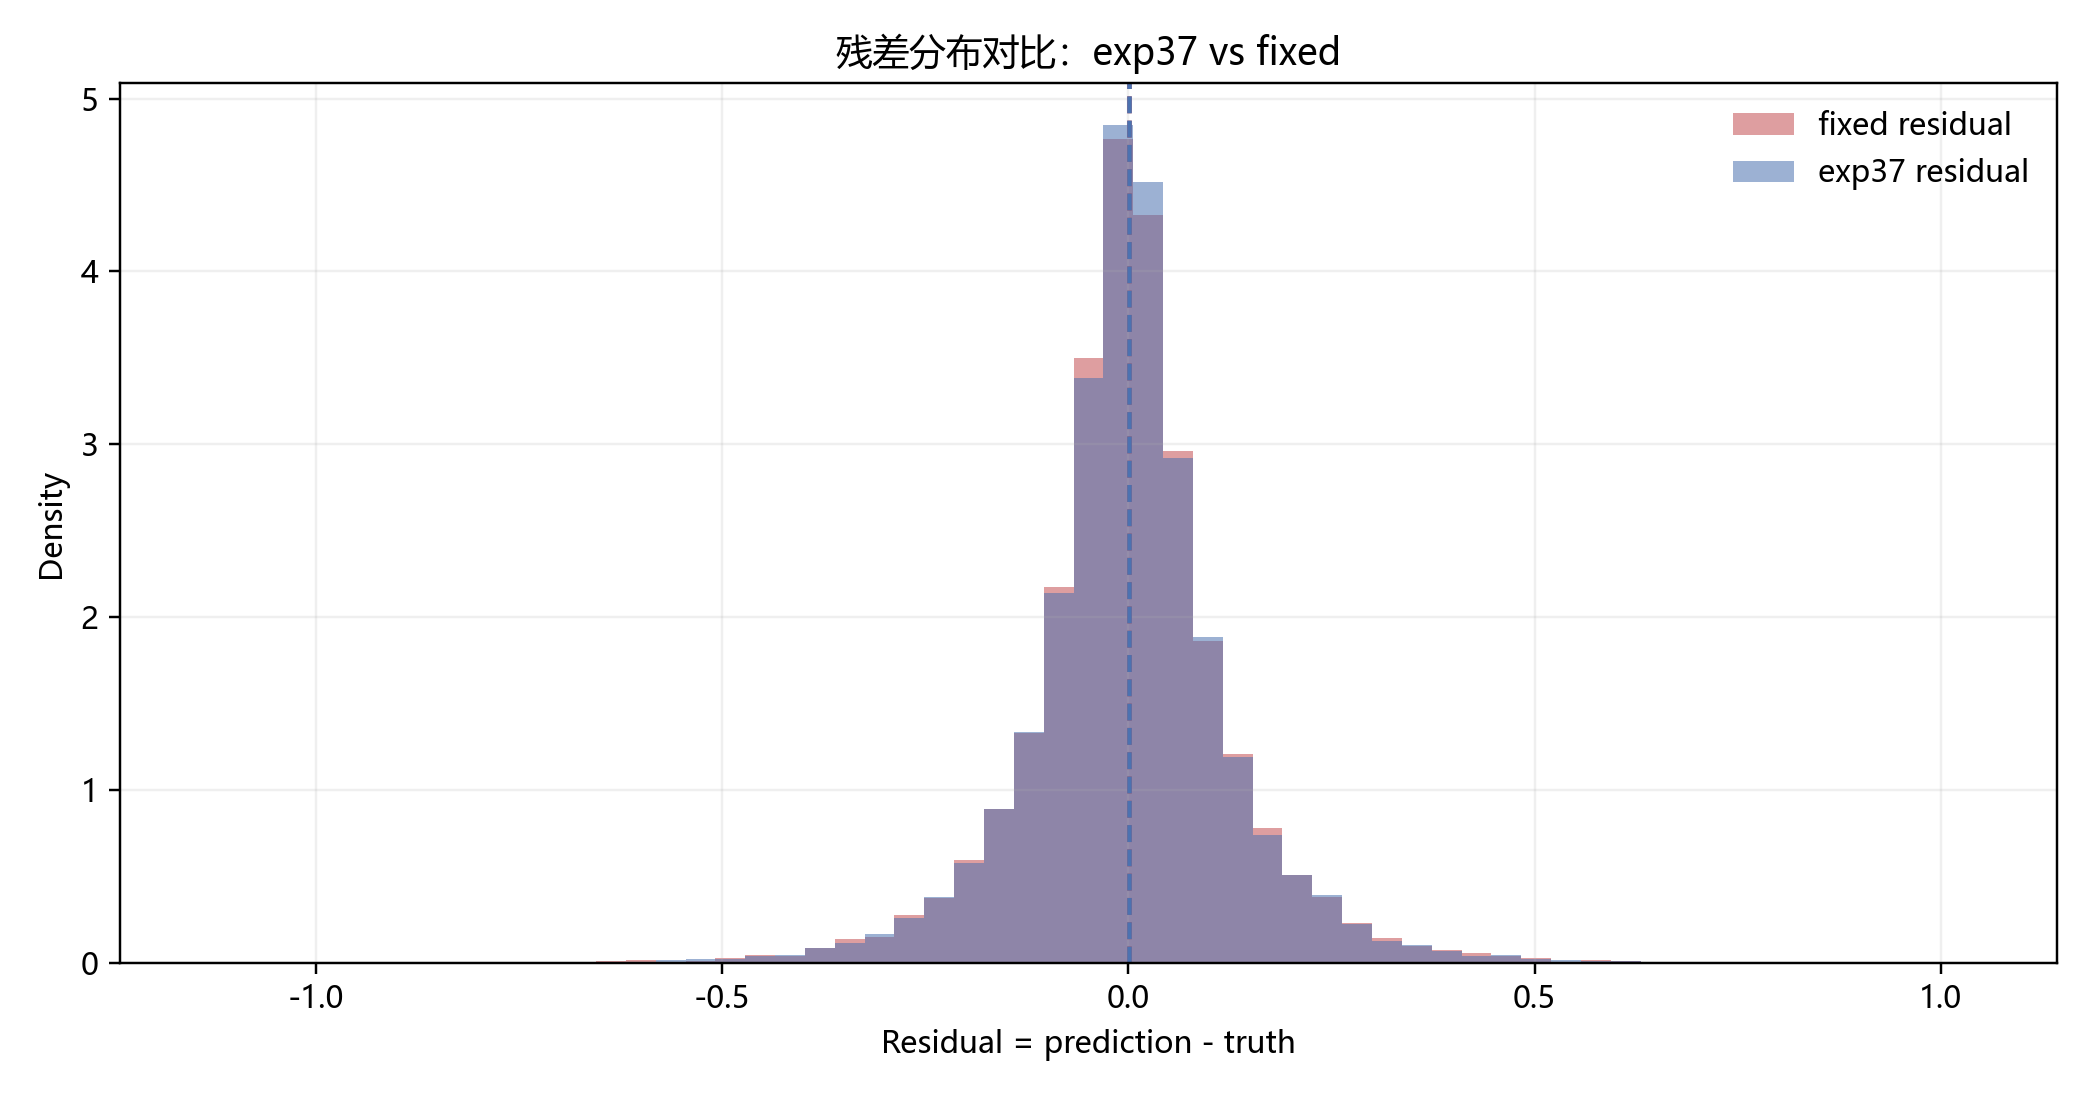
\includegraphics[width=0.92\linewidth]{figures/exp37_residual_distribution.png}
\caption{exp37 与 fixed 的残差分布对比。}
\label{fig:residual}
\end{figure}

图 \ref{fig:residual} 给出了残差分布的进一步证据。可以看到，exp37 的残差中心更接近零点，分布宽度也更窄，这说明该方法不仅降低了绝对误差，也在一定程度上减少了系统性偏差和大范围波动。定量上，残差均值由 `fixed` 的 $7.08\times 10^{-4}$ 收缩到 $5.59\times 10^{-4}$，残差标准差由 $0.12873$ 收缩到 $0.12698$。对评估一个同化方法是否真正稳定来说，这比单独看 RMSE 更有解释力。

\begin{figure}[htbp]
\centering
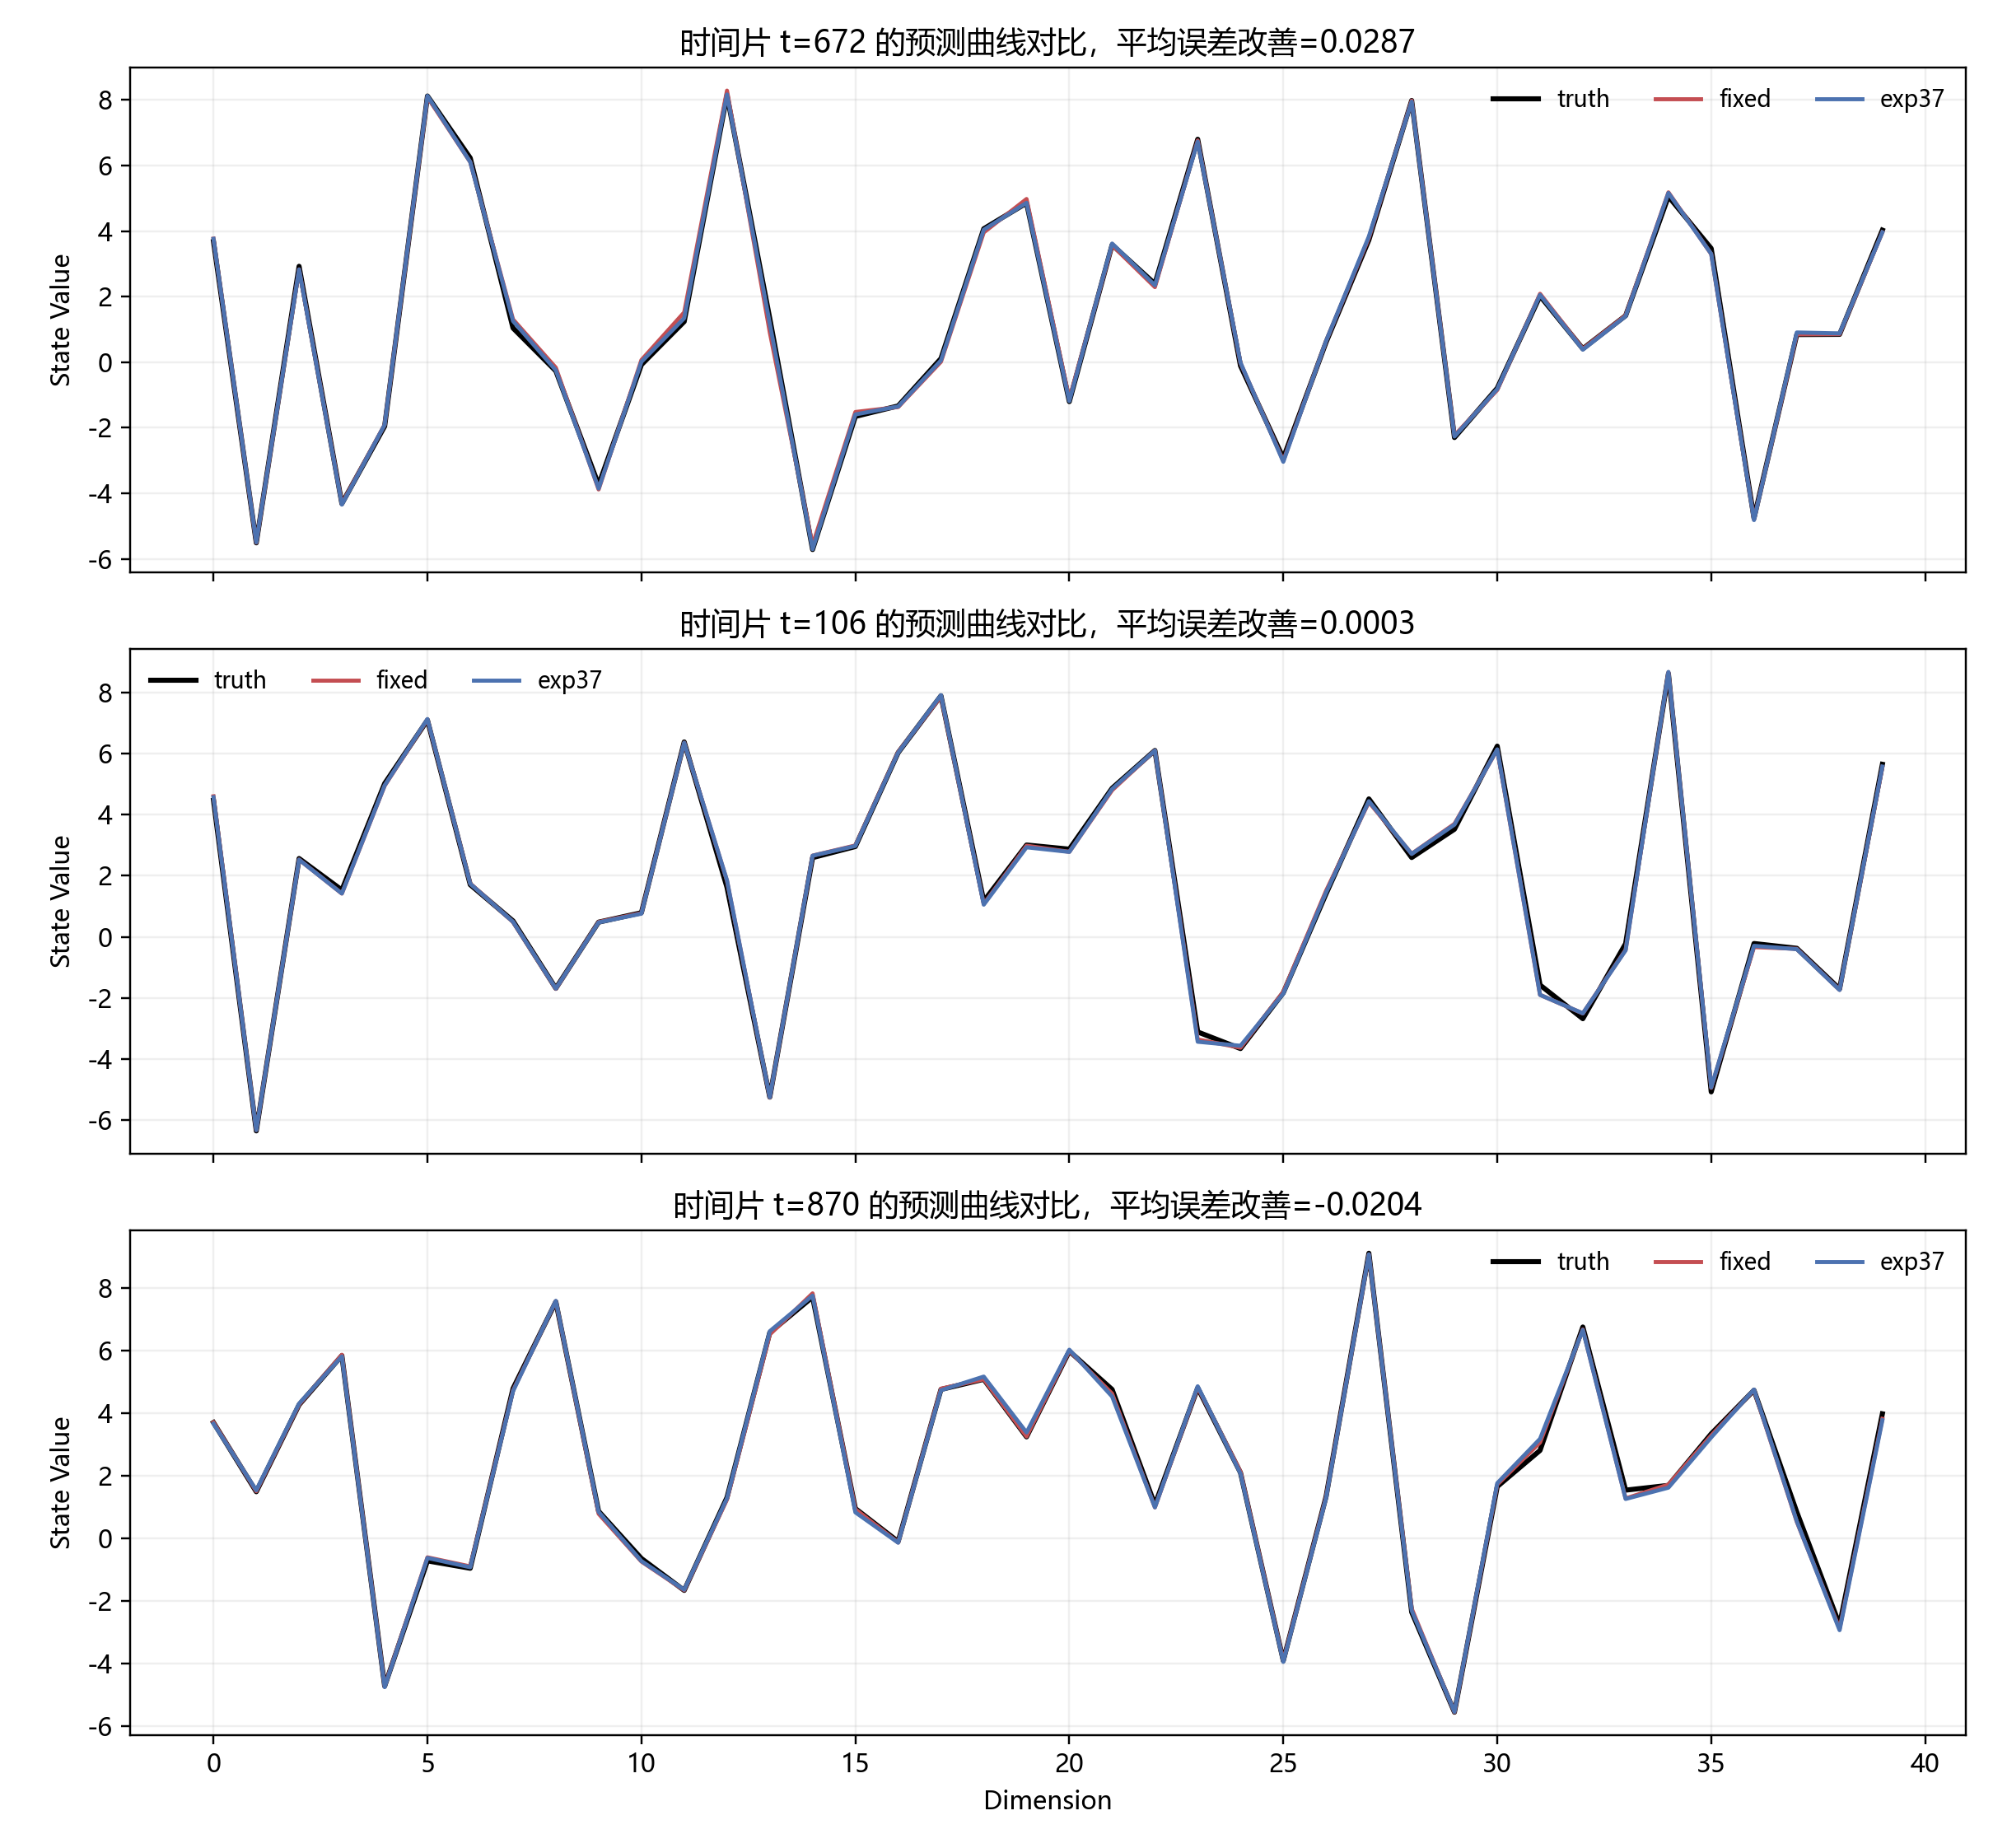
\includegraphics[width=0.92\linewidth]{figures/exp37_case_slices.png}
\caption{代表性时间片上 truth、fixed 与 exp37 的状态切片对比。}
\label{fig:slices}
\end{figure}

最后，图 \ref{fig:slices} 给出了最直观的状态切片对比。相比 fixed，exp37 在若干代表性时间片上对峰值、谷值以及局地转折位置的跟踪更贴近真实曲线。这说明量子弱融合带来的并不是抽象指标上的微小变化，而是对局地状态形状恢复能力的实际增强。对于论文报告而言，这类图尤为重要，因为它把“量子结构信息改善了局地几何重建”这一核心故事，转化成了可直接观察的证据。

\begin{figure}[htbp]
\centering
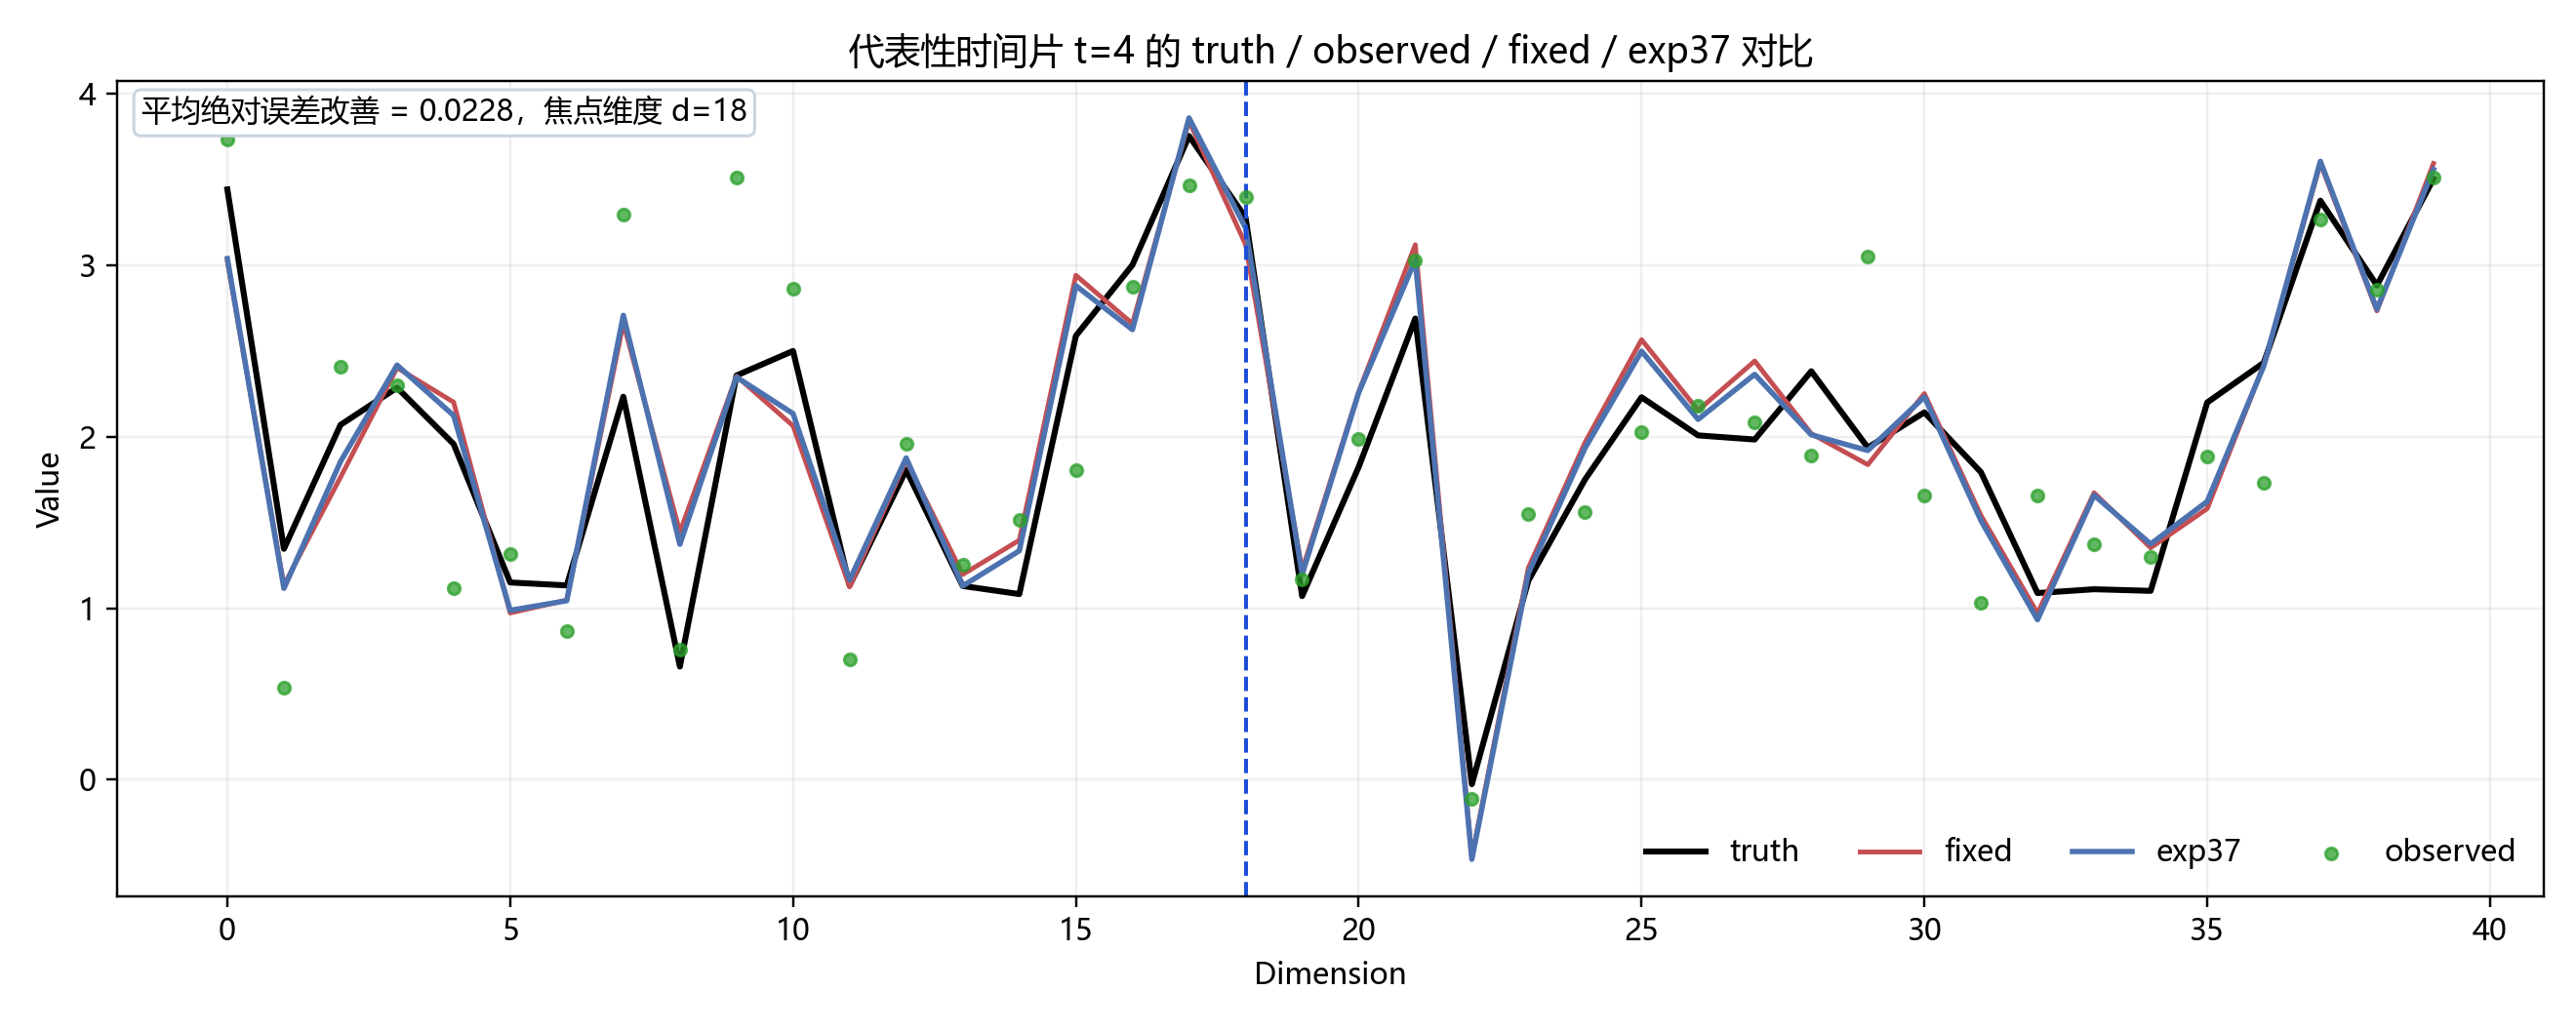
\includegraphics[width=0.92\linewidth]{figures/exp37_observed_truth_fixed_best_slice.png}
\caption{代表性高收益时间片上 observed、truth、fixed 与 exp37 的状态切片对比。}
\label{fig:obs-slice}
\end{figure}

图 \ref{fig:obs-slice} 则把观测值也引入了比较。这样做的好处是，可以区分“更贴近观测”和“更贴近真实状态”这两件事。在带噪观测条件下，一个方法如果只是过度追随观测，不一定意味着同化更好；而图 \ref{fig:obs-slice} 显示，exp37 在关键时间片上既没有简单复制带噪观测，也没有停留在 fixed 的平均化趋势上，而是在二者之间更好地恢复了真实曲线形态。定量上，该代表性高收益时间片对应 $t=672$，此时 `fixed` 的切片 RMSE 为 $0.1229$，最优量子方案为 $0.0781$，单时间片下降约 $36.5\%$。这一图直接体现了数据同化任务中最重要的能力，即在模型和观测之间找到更合理的平衡点。
